
% Szakdolgozat, diplomaterv esetén a dolgozat felépítése valami ehhez hasonló, témától függetlenül lehet természetesen eltérés:
% -Bevezetés, 1-2 oldal, a téma elhelyezése, miről lesz szó
% -Szakirodalmi áttekintés: a dolgozat kb harmada, szükséges előismereteket tartalmazza, illetve szakdolgozat esetén kb 5, diplomaterv esetén kb 10 szakmai cikk hivatkozása, 
%   1-1 bekezdésben összefoglalva, kik, mivel mit csináltak, milyen eredményre jutottak, az aktuális dolgozathoz hogy kapcsolódik, 
%   miért releváns. Kutatós témák esetén ez lényegesen nagyobb hangsúlyt kap (több cikk is hivatkozható!), 
%   fejlesztős feladatok esetén hasonló termékek bemutatása, elmélet amire a tervezés (a későbbiekben bemutatandó munka) épül.
% -Tervezés (témától függően más is lehet a fejezet címe): A saját munka bemutatása. Hardver fejlesztős dolgozat esetén kapcsolási rajz részletek megmagyarázva stb.
% -Értékelés: Szimulációs eredmények, valós mérések bemutatása, a megvalósítás mennyire sikerült, eltérések a várttól.
% -Összefoglalás: a dolgozat összefoglalása, kb 1-2 oldal, jövőbeli tervek.
% A szakirodalmakhoz lehet használni guglit, de ne ez legyen az első. Tanszéki és kolis hálóról elérhetőek online folyóiratok, ez a legjobb forrás (gugli is indexel) pl:
% -IEEE Xplore
% -Elsevier
% -Springerlink
% (-Google scholar)
% -stb
% A wikipedia, youtube és online hírportálok hivatkozását lehetőleg mindenki kerülje. Ha mégis nagyon releváns, ők is hivatkozni szoktak az eredeti forrásra, azt nézzétek meg.
% Szakirodalmak feldolgozása:
% -Absztrakt elolvasása, el kell dönteni, hogy releváns-e a cikk vagy sem
% -Bevezetés átolvasása, általában egy jó áttekintése a témakörnek
% -Ábrák átnézése
% -Conclusion rész elolvasása
% -Aki jobban el akar merülni benne, a többi rész is elolvasható
% -Ezek alapján néhány mondatos összefoglaló generálása

% Hasonló rendszerek
% https://esphome.io/
% https://www.openhab.org/
% Kész termékek
% https://www.itead.cc/sonoff-pow.html

%mqtt https://ieeexplore.ieee.org/abstract/document/4554519
%smarthome + nodered https://ieeexplore.ieee.org/document/8603575
%titkosítások összehasonlítása https://ieeexplore.ieee.org/abstract/document/8822208

\chapter{Szakirodalmi áttekintés}
\section{ESP8266}
Az egységek alapja egy az Espressif cég által gyártott mikrokontroller, amelyen található egy 32bit-es 80Mhz-es Tensilica processzor, 50kB RAM, egy külső flash chip. Az utóbbi flash felelős felhasználói program tárolásért. Emellett megvalósításra került egy teljes WiFi stack-et, amely támogatja a 802.11 b/g/n szabványokat. A modulnak két virtuális WiFi interfésze van, amikkel tudja biztosítani, hogy állomásként (station), elérési pontként (softAP) vagy egyszerre mind a két módon üzemeljen. Az utóbbi tulajdonság segítségével lehet Mesh hálózatokat létrehozni.

\begin{figure}[!ht]
    \centering
    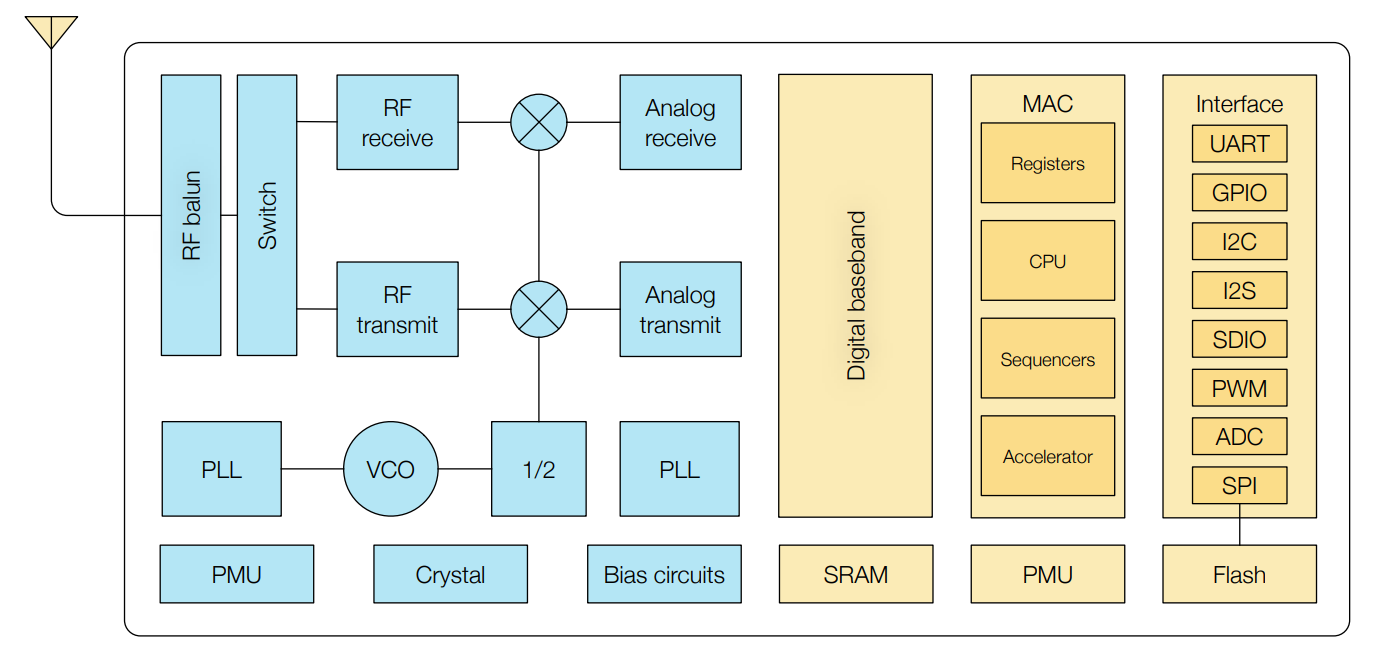
\includegraphics[width=150mm, keepaspectratio]{figures/esp8266funcdiag.png}
    \caption{Az ESP8266 funkcionális diagramja}
    \label{fig:TeXstudio}
\end{figure}

A ESP8266-hoz léteznek különböző típusú moduljai (pl. ESP-01, ESP-12). Az eltérés a modulok között általában a panelre kivezetett GPIO szám és a modul mérete jelenti. Összesen 17 db GPIO láb áll rendelkezésre, amelyekhez különböző funkciók rendelhetők. Szoftveresen beállítható egy kivételével mindegyik lábra interupt. Rendelkezik 2db UART, 3db SPI és szoftveresen beállítható I2C interfésszel is.
Az IoT rendszerekben és távol vezérlésű rendszerekben népszerűen használják, ami elsősorban az alacsony árának és a vele kompatibilis fejlesztői környezetnek (pl. Arduino, VStudio) is köszönhető. Rengeteg előre elkészített könyvtár található hozzá, amikkel gyorsan lehet például prototípusokat elkészíteni. A gyártó alapvetően 3 különböző SDK-t biztosít a fejlesztéshez. Az Arduino core-t, NONOS SDK-t, illetve a RTOS SDK-t. Az utóbbi egy FreeRTOS alapú operációs rendszer.

Számos versenytársa létezik például a RTL8710, AIR602 amik eltérő processzort használnak, de alapvető tulajdonságaikban nincs nagy eltérés. Ezenkívűl létezik már az 8266-nak egy újabb verziója az ESP32, ami már 2-magos processzorral, nagyobb memóriával és több perifériával rendelkezik.

% http://wiki.seeedstudio.com/W600_Module/
% különböző modul típusok
% elérhető lábszám
% alacsony ár
% miben lehet rá fejleszteni
% iotban elterjedt, hasonló ellenfele RTL8710


\section{ESPNOW}
Az ESPNOW egy kommunikációs protokoll, ami WiFi-hez hasonlóan a 802.11-es szabvány alapján működik. Az egyik eltérés a WiFi-hez képest, hogy nincs külön kapcsolat felépítés az eszközök között. Ennek köszönhetően kevesebb az overhead a kommunikáció során, és így kissebek az átküldött csomagok mérete.

A fizikai és hozzáférési réteg felett a gyártó által definiált egyedi keret található. A frame tartalmaz egy Body mezőt, ami tartalmazhatja az alkalmazásunk payload-ját. Ennek a mérete 0-250 byte között változhat. A keret ezenkívűl tartalmaz még számos a gyártó által használt mezőt, mint pl ESPNOW verziószámát, egyedi azonosítót, ami az adott ESP MAC címének az első 3 bájtja alkot.

\begin{table}[ht]
	\footnotesize
	\centering
	\begin{tabular}{ | c | c | c | c | c | c |}
		\toprule
		Egység ID & Méret & Azonosító &  Típus & Verzió & Body \\
		\midrule
        1 bájt & 1 bájt & 3 bájt & 1 bájt & 1 bájt & 0-250 bájt \\
	\end{tabular}
	\caption{ESPNOW keretformátum}
	\label{tab:TabularExample}
\end{table}

Az adatküldés előtt az egységeket párosítani kell egymáshoz. Ez az inicializálás során történhet meg egyszerűen a másik eszköz softAP interfészének MAC címét megadva. Lehetség van tovább broadcast üzeneteket is küldeni az azonos csatornán lévő eszközöknek. Ebben az esetben a párosítás során a broadcast FF:FF:FF:FF:FF:FF címet is hozzá kell adni. Lehetőség van a 2.4ghz sávban található 14db WiFi csatorna használatára. Egy modul maximum 20 másik eszközzel lehet összepárosítva. Lehetőség van tovább kiküldött keretek titkosítására is ez AES-128 algoritmus használatval történik. Lehetőség van tovább egyszerre egy normál routerre, illetve az ESPNOW-t is használni, egy olyan feltétellel hogy megkell egyezni a használt csatornánank.

% nincs külön kapcsolat két eszköz között
% custom frame format
% sikeres küldés esetén ack, TODO mérni kellene
% https://docs.espressif.com/projects/esp-idf/en/latest/api-reference/network/esp_now.html

\section{MQTT}

% Az MQTT egy publikáló-feliratkozó protokoll, amely főleg az IoT-ban is használt kis teljesítményű eszközökre lett tervezve. Előnyeihez tartozik továbba, hogy jól használható alacsony sávszélesség esetb 

\section{NodeRED}
% https://nodered.org/

\section{Home Assistant}
% https://www.home-assistant.io/

\section{ESPHome}
% https://esphome.io/

\section{Openhab}

% https://ieeexplore.ieee.org/document/8603575